\subsection*{Solution to Spring 2013, \#1}\label{s131}
Taking the Fourier transform, we have $\wh{u}_{t} = t^{2}(-4\pi^{2}|\xi|^{2})\wh{u}.$
Thus
$\wh{u}(\xi, t) = \wh{g}(\xi)e^{-\frac{4}{3}\pi^{2}|\xi|^{2}t^{3}}.$
Therefore
$u(x, t) = g(x) \ast [e^{-\frac{4}{3}\pi^{2}|\xi|^{2}t^{3}}]^{v}$.
Note that $e^{-\frac{4}{3}\pi^{2}|\xi|^{2}t^{3}}$ is a Schwarz function in $\xi$. Since the Fourier inverse of $e^{-\pi|\xi|^{2}/a}$ is $e^{-\pi a|x|^{2}}a^{n/2}$
for $a > 0$, it follows that
\begin{align*}
[e^{-\frac{4}{3}\pi^{2}|\xi|^{2}t^{3}}]^{v} = e^{-\frac{3}{4}t^{-3}|x|^{2}}(\frac{3}{4\pi}t^{-3})^{n/2}.
\end{align*}
Therefore
$u(x, t) = g(x) \ast e^{-\frac{3}{4}t^{-3}|x|^{2}}(\frac{3}{4\pi}t^{-3})^{n/2}$ is continuous in $t > 0$ for each fixed $x$.

Since $e^{-\frac{4}{3}\pi^{2}|\xi|^{2}t^{3}} \leq 1$ for all $\xi, t$, $$\nms{\wh{u}(\xi, t)}_{L^{2}_{\xi}}^{2} \leq \nms{\wh{g}}_{L^{2}_{\xi}}^{2} < \infty$$
and hence $\wh{u}(\xi, t) \in L^{2}_{\xi}$. Therefore $u(x, t) \in L^{2}_{x}$.
Finally,
\begin{align*}
\nms{u(x, t) - g(x)}_{L^{2}_{x}}^{2} = \nms{\wh{u}(\xi, t) - \wh{g}(\xi)}_{L^{2}_{\xi}}^{2} = \int_{\R^{n}}|\wh{g}(\xi)|^{2}|e^{-\frac{4}{3}\pi^{2}|\xi|^{2}t^{3}} - 1|^{2}\, d\xi \rightarrow 0
\end{align*}
as $t \rightarrow 0^{+}$ by the Dominated Convergence Theorem and the fact that $\wh{g} \in L_{\xi}^{2}$. \hfill\qed

\subsection*{Solution to Spring 2013, \#2}\label{s132}
By Duhamel's principle,
\begin{align*}
u(x, t) = \frac{1}{2}(\vp(x + t) + \vp(x - t)) + \frac{1}{2}\int_{x - t}^{x + t}\psi(s)\, ds -\frac{1}{2}\int_{0}^{t}\int_{x - (t - s)}^{x + (t -s)}C(y, s)u(y, s)\, dy\, ds.
\end{align*}
For $|x| > R + t$, by how the support of $\vp$, $\psi$, and $C$ is defined, it follows that $u(x, t) = 0$ for $|x| > R + t$.
\hfill\qed

\subsection*{Solution to Spring 2013, \#3}\label{s133}
\subsubsection*{Solution to $3a$}
Since $u$ is a solution to $-\Delta u + u^{1/3} = 0$ in $D$ and $u = 0$ on $\pr D$,
\begin{align*}
0 = \int_{D}-u\Delta u + u^{4/3}\, dx = \int_{D}\abn{\nabla u}^{2} + u^{4/3}\, dx
\end{align*}
where the last equality is by integration by parts.
Therefore
\begin{align*}
0 \leq \int_{D}u^{4/3}\, dx = -\int_{D}\abn{\nabla u}^{2}\, dx = 0
\end{align*}
which implies that $\nabla u = 0$ (almost everywhere) in $D$. Since $u = 0$ on $\pr D$,
it follows that $u - 0$ in $D$.
\hfill\qed

\subsubsection*{Solution to $3b$}
We prove that the problem as stated is false. (For the possibly intended solution, see the end of this proof.)
For all $u \in H_{0}^{1}(D)$, let
$$I[u] := \frac{1}{2}\int_{D}|\nabla u|^{2}\, dx - \frac{3\alpha}{4}\int_{D}|u|^{4/3}\, dx.$$
Note that since $u \in H_{0}^{1}(D)$, $u \in L^{4/3}(D)$ by Holder's inequality and so $I[u]$ is well defined.
A calculus of variations argument shows that the minimizer of $I[u]$ over $u \in H_{0}^{1}(D)$ (if it exists)
will satisfy the PDE stated in the problem. We will prove the existence of such a minimizer and
that this minimizer is not the zero function independent of the smallness of $\alpha$.

By Holder's inequality and Poincare's inequality, for all $u \in H_{0}^{1}(D)$,
\begin{align*}
\int_{D}|u|^{4/3}\, dx \leq |D|^{1/3}\bigg(\int_{D}|u|^{2}\, dx\bigg)^{2/3} \leq C_{D}\bigg(\int_{D}|\nabla u|^{2}\, dx\bigg)^{2/3}
\end{align*}
for some constant $C_{D}$ depending only on the domain $D$. Thus
$$I[u] \geq \frac{1}{2}\nms{\nabla u}_{L^{2}(D)}^{2} - \frac{3\alpha}{4}C_{D}\nms{\nabla u}_{L^{2}(D)}^{4/3}.$$
Let $L(p, z, x) := \frac{1}{2}|p|^{2} - \frac{3\alpha}{4}|z|^{4/3}$. Since $L$ is convex in $p$,
by the proof of Theorem 2 on Page 470 of Evans (in the proof, the only place where a lower bound on $I$ was used was to show that $\sup_{k}\nms{Du_{k}}_{L^{q}(U)} < \infty$ but this is still the case),
there exists at least one $\wt{u} \in H_{0}^{1}(D)$ such that $I[\wt{u}] = \min_{u \in H_{0}^{1}(D)}I[u]$.
This $\wt{u}$ is a solution to the given PDE. We now show that it is nontrivial.

Let $w \in H_{0}^{1}(D)$. For some $0 < a < 1/100$ to be chosen later, we compute
\begin{align*}
I[aw] = \frac{a^{2}}{2}\int_{D}|\nabla w|^{2}\, dx - \frac{3\alpha a^{4/3}}{4}\int_{D}|w|^{4/3}\, dx = C_{1, w}a^{2} - C_{2, w}a^{4/3} < 0
\end{align*}
if $a$ is chosen to be sufficiently small (depending on $w$). With this choice of $a$, $aw \in H_{0}^{1}(D)$ and hence
\begin{align*}
I[\wt{u}] \leq I[aw] < 0 = I[0].
\end{align*}
Therefore $\wt{u}$ cannot be the zero solution. Thus regardless of how small $\alpha$ is, we cannot have the solution $u$ be identically zero.
\hfill\qed

\begin{rem}
The following is probably the intended solution, due to Stephanie Wang. Let $u \in H_{0}^{1}(D)$ such that
$\Delta u + \alpha u^{1/3} = 0$. Then integration by parts yields
\begin{align}\label{s133beq1}
0 = \int_{D}u\Delta u + \alpha u^{4/3}\, dx = \int_{D}\alpha u^{4/3} - \abn{\nabla u}^{2}\, dx.
\end{align}
From Poincare's Inequality, there exists a constant $C$ depending only on $D$ such that
\begin{align*}
\int_{D}u^{2}\, dx \leq C\int_{D}|\nabla u|^{2}\, dx = C\int_{D}\alpha u^{4/3}\, dx \leq C\alpha\bigg(\int_{D}u^{2}\, dx\bigg)^{1/2}\bigg(\int_{D}u^{2/3}\, dx \bigg)^{1/2}
\end{align*}
where the first equality is by an application of \eqref{s133beq1} and the last inequality is by an application of
Cauchy-Schwarz.
Therefore
$$\int_{D}u^{2}\, dx \leq (C\alpha)^{2}\int_{D}u^{2/3}\, dx.$$
Since $x^{2/3} \leq \max(x^2, 1)$, combining this with the above equation yields
$$\int_{D}u^{2}\, dx \leq (C\alpha)^{2}|D| + (C\alpha)^{2}\int_{D}u^{2}\, dx$$
where $|D| = \int_{D}1\, dx$.
Thus for $\alpha$ small enough so that $1 - (C\alpha)^{2} > 0$, rearranging yields
\begin{align*}
\int_{D}u^{2}\, dx \leq \frac{(C\alpha)^{2}|D|}{1 - (C\alpha)^{2}}.
\end{align*}
It is now tempting to let $\alpha \rightarrow 0$, however, we cannot do this since we recall that $u$ also depends on $\alpha$.
\hfill\qed
\end{rem}

\subsection*{Solution to Spring 2013, \#4}\label{s134}
We present two solutions to Problem $4a$, first we present an ``energy" approach and then present a maximum principle approach.
\subsubsection*{Solution to $4a$ - Energy}
We have
\begin{align*}
0 = \int_{\R^{n}}u\Delta u - q(x)u^{2}\, dx = \int_{\R^{n}}-|\nabla u|^{2} - q(x)u^{2}\, dx.
\end{align*}
Therefore
$$0 \leq \int_{\R^{n}}|\nabla u|^{2}\, dx = \int_{\R^{n}}-q(x)u^{2}\, dx \leq 0$$
where the last inequality is because $q(x) \geq 0$. Therefore
$$\int_{\R^{n}}|\nabla u|^{2}\, dx = 0$$ which implies that $u$ is a constant. Since $u \rightarrow 0$ uniformly when $|x| \rightarrow \infty$, it follows
that $u \equiv 0$.
\hfill\qed

\subsubsection*{Solution to $4a$ - Maximum Principle}
Let $\delta> 0$. Because $u(x) \to 0$ uniformly as $|x| \to \infty$, we may find $R>0$ such that $|u(x)| \leq \delta$ on $\d B_R(0)$. Now, consider
\[
\left\{
\begin{array}{ll}
	\Delta u - q(x) u = 0 & \text{in} \,\,\, B_R(0)\\
	|u(x)| \leq \delta & \text{on} \,\,\, \d B_R(0)
\end{array}
\right.
\]
where $q(x) \geq 0$ is bounded. Define $v := u - \delta$, which implies $v$ satisfies
\[
\left\{
\begin{array}{ll}
	\Delta v - q(x) v = q(x) \delta \geq 0 & \text{in} \,\,\, B_R(0) \\
	v \leq 0 & \text{on} \,\,\, \d B_R(0)
\end{array}
\right.
\]
Let $\tilde{R}> R$, $\epsilon >0$, and define $w := v + \epsilon(|x|^2- \tilde{R}^2)$. (The perturbation $w = v + \epsilon e^{\lambda x_1}$ would work as well.) Then, in $B_R(0)$,
$$ \Delta w - q(x) w = \Delta v + 2n\epsilon - q(x) v - \epsilon q(x) (|x|^2 - \tilde{R}^2) > 0$$
so $w$ satisfies
\begin{equation}
\left\{
\begin{array}{ll}
	\Delta w - q(x) w > 0 & \text{in} \,\,\, B_R(0) \\
	w < 0 & \text{on} \,\,\, \d B_R(0)
\end{array}
\right.
\end{equation}
Because $u$ is at least twice differentiable, $u$, and thus $w$, are continuous. Hence, $w$ must attain a maximum in $\overline{B_R(0)}$. Suppose $w$ attains a positive maximum at $x_0$. Because of the boundary condition of $w$, $x_0$ must be in the interior. It follows that
$$ \Delta w(x_0) - q(x_0) w(x_0) \leq 0 $$
which is a contradiction to (1). Thus, any maximum of $w$ must be nonpositive, so $w \leq 0$ in $B_R(0)$. Running through the same argument with $v := u + \delta$ and $w$ replaced by $-w$ will yield $w \geq 0$ in $B_R(0)$. Hence, $w \equiv 0$ in $B_R(0)$. This holds for all choice of $\epsilon > 0$, so sending $\epsilon$ to zero yields $v \equiv 0$ in $B_R(0)$. Thus, $u \equiv \delta$ in $B_R(0)$. This holds for all $\delta > 0$, and sending $\delta$ to 0 implies taking $R$ to $\infty$, so we arrive at $u \equiv 0$ on $\R^n$.
\hfill\qed

\subsubsection*{Solution to 4b}

Recall that $\Delta u$ in radial coordinates in $\R^n$ is
$$ \Delta u = u''(r) + \frac{n-1}{r} u'(r) $$
Hence, we need to solve the ODE
$$ u''(r) + \frac{2}{r} u'(r) + u(r) = 0 $$
where $u(r) \to 0$ as $r \to \infty$. Multiplying the ODE through by $r^2$ yields
$$ r^2 u'' + 2r u' + r^2 u = (r^2 u')' + r^2 u = 0 $$
The fact that the ODE is now in this form implies that using the substitution $v = \sqrt{r^2}u = ru$ might be a worthwhile substitution. Indeed,
$$ v' = ru' + u, \quad \quad v'' = ru'' + 2u' $$
which means, if we multiply the original ODE through by $r$, we have
$$ ru'' + 2u' + ru = v'' + v = 0 $$
Solving the ODE for $v$ yields
$$ v(r) = A\sin(r) + B\cos(r) $$
Thus,
$$ u(r) = A \frac{\sin(r)}{r} + B \frac{\cos(r)}{r} $$
Observe that this $u$ satisfies the condition $u(r) \to 0$ as $r \to \infty$. \hfill\qed

\subsection*{Solution to Spring 2013, \#5}\label{s135}
There's a small error with the problem statement. It should read ``show that any \emph{nonzero} solution..." The zero solution is an equilibrium point of the system, so that solution will not be converging to the unit circle. With this in mind, we convert to polar coordinates to make this problem really easy. Let $r^2 = y_1^2 + y_2^2$ and $\tan (\theta) = y_2/y_1$. Then,
\begin{align*}
r^2 = y_1^2 + y_2^2 \quad &\implies \quad 2r\dot r = 2 y_1 \dot y_1 + 2 y_2 \dot y_2 \\
&\implies \quad r \dot r = y_1 y_2 + y_2 (-y_1 + (1 - y_1^2 - y_2^2)y_2) \\
&\implies \quad r \dot r = (1-r^2)r^2 \sin^2 (\theta) \\
&\implies \quad \dot r = (1-r^2) r \sin^2 (\theta)
\end{align*}
It follows that if $0<r<1$, then $\dot r > 0$, and if $r > 1$, then $\dot r < 0$. Moreover, if $r=1$, then $\dot r = 0$. This implies that all solutions to the converge to the unit circle. Furthermore,
\begin{align*}
\tan (\theta) = \frac{y_2}{y_1} \quad &\implies \quad \sec^2 (\theta) \dot \theta = \frac{y_1 \dot{y}_2 - y_2 \dot{y_1}}{y_1^2} \\
&\implies \quad \sec^2 (\theta) \dot \theta = \frac{y_1 (-y_1 +(1-y_1^2 + y_2^2)y_2) - y_2^2}{y_1^2} \\
&\implies \quad \sec^2 (\theta) \dot \theta = \frac{-r^2 + r^2 \sin(\theta) \cos(\theta) (1-r^2)}{r^2 \cos^2(\theta)} \\
&\implies \quad \dot \theta = -1 + \sin(\theta) \cos(\theta) (1-r^2)
\end{align*}
Observe that as $r \to 1$ (which we get from the ODE for $r$ above), then $\dot \theta \to -1$. This means that as solutions converge to the unit circle, they will be circling in the clockwise direction. Thus, any nonzero solution of the system converges to $(\sin(t+c),\cos(t+c))$ as $t \to \infty$ for some constant $c$.  \qed

\subsection*{Solution to Spring 2013, \#6}\label{s136}
The equilibrium points are when $x(2 - x -y ) = 0$ and $y(3 - 2x - y) = 0$. This occurs when
$(x, y) = (0, 0), (0, 3), (2, 0)$, and $(1, 1)$. The Jacobian is
$$J(x, y) = \pmat{2 - 2x - y}{-x}{-2y}{3 - 2x - 2y}.$$

At $(0, 0)$, the Jacobian is $\smat{2}{0}{0}{3}$ which has eigenvalues $2, 3$ with corresponding eigenvectors $\svt{1}{0}$ and ${0}{1}$.

At $(0, 3)$, the Jacobian is $\smat{-1}{0}{-6}{-3}$ which has eigenvalues $-1, -3$ with corresponding eigenvectors $\svt{-3}{1}$ and ${0}{1}$.

At $(2, 0)$, the Jacobian is $\smat{-2}{-2}{0}{-1}$ which has eigenvalues $-2$, $-1$ with corresponding eigenvectors $\svt{1}{0}$ and ${-2}{1}$.

At $(1, 1)$, the Jacobian is $\smat{-1}{-1}{-2}{-1}$ which has eigenvalues $-1 \pm \sqrt{2}$ with corresponding eigenvectors $\svt{\mp\sqrt{2}/2}{1}$.

The phase portrait is as follows:
\begin{center}
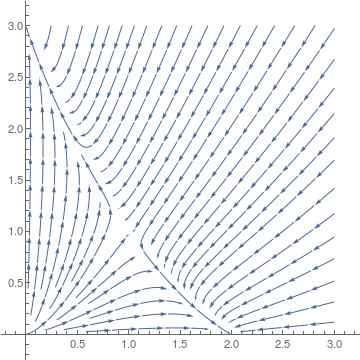
\includegraphics[scale = 0.75]{./_Figures/S13Q6.png}
\end{center}
\noindent From the phase portrait, it is not likely that both species will survive.
\hfill\qed

\subsection*{Solution to Spring 2013, \#7}\label{s137}
We give two solutions. The first is an application of the Cole-Hopf transformation, the second is a direct proof using the maximum principle.

Suppose $u$ solves the given PDE. Let $w := e^{-u}$. Then $w_{t} = -e^{-u}u_{t}$ and $\Delta w = e^{-u}|\nabla u|^{2} - e^{-u}\Delta u$.
Thus in $\Om \times (0, \infty)$,.
$$w_{t} - \Delta w = -e^{-u}u_{t} - e^{-u}|\nabla u|^{2} + e^{-u}\Delta u = -e^{-u}(u_{t} + |\nabla u|^{2} - \Delta u) = 0.$$
It follows that $w$ satisfies
\begin{align}\label{s137eq1}
\begin{cases}
w_{t} - \Delta w = 0 & \text{ in } \Om \times (0, \infty)\\
w(x, t) = e^{-g(x)} & \text{ on } \pr\Om \times (0, \infty)\\
w(x, 0) = e^{-f(x)} & \text{ in } \Om.
\end{cases}
\end{align}
Suppose $w_{1}$ and $w_{2}$ were two distinct solutions to \eqref{s137eq1}. Then let $v := w_{1} - w_{2}$. We have
\begin{align*}
\begin{cases}
v_{t} - \Delta v & \text{ in } \Om \times (0, \infty)\\
v(x, t) = 0 & \text{ on } \pr\Om \times (0, \infty)\\
v(x, 0) = 0 & \text{ in } \Om.
\end{cases}
\end{align*}
Let $E(t) := \frac{1}{2}\int_{\Om}v(x, t)^{2}\, dx$. Then
$$\dot{E}(t) = \int_{\Om}vv_{t}\, dx = \int_{\Om}v\Delta v\, dx = -\int_{\Om}|\nabla v|^{2}\,dx \leq 0.$$
Therefore $v \equiv 0$. Thus the solution to \eqref{s137eq1} is unique. Suppose $u_{1}$, $u_{2}$ were two distinct
solutions to the stated PDE in the problem. Then $w_{1} := e^{-u_{1}}$ and $w_{2} := e^{-u_{2}}$ are two distinct
solutions to \eqref{s137eq1}, a contradiction. Therefore the solution to the stated PDE is unique.

We now present a maximum principle approach.
Suppose both $u$ and $v$ satisfy the PDE where $u \neq v$, and consider $w := u-v$. Fixing $T > 0$, observe that $w$ satisfies the following PDE:
\[
\left\{
\begin{array}{ll}
	w_t - \Delta w + |\del u|^2 - |\del v|^2 = 0 & \text{in} \,\,\, \Omega \times (0,T)\\
	w = 0 & \text{on} \,\,\, \d \Omega \times (0,T) \\
	w(x,0) = 0 & \text{in} \,\,\, \Omega
\end{array}
\right.
\]
Now, define $y = w - \epsilon t$, and observe
\begin{equation}
\label{one}
	y_t - \Delta y + |\del u|^2 - |\del v|^2 = - \epsilon < 0, \quad \quad \text{in} \,\,\, \Omega \times (0,T)
\end{equation}
Because $u$ and $v$ are at least twice differentiable, $w$, and thus $y$, are continuous. It follows that $y$ must attain a maximum at $(x_0,t_0) \in \overline{\Omega} \times [0,T]$. Suppose $(x_0,t_0) \in \Omega \times (0,T)$ (the interior). This would imply
$$y_t(x_0,t_0) = 0, \quad \quad \Delta y(x_0,t_0) \leq 0$$
and
$$\del y(x_0,t_0) = \del w(x_0,t_0) = \del u(x_0,t_0) - \del v(x_0,t_0) = 0 \quad \implies \quad \del u(x_0,t_0) = \del v(x_0,t_0) $$
($\del u$ and $\del v$ must exist everywhere, even at the boundary, since $u$ and $v$ are smooth on the boundary.) Hence,
$$ (y_t - \Delta y + |\del u|^2 - |\del v|^2)(x_0,t_0) = - \Delta y(x_0,t_0) \geq 0 $$
which contradicts \eqref{one}. Hence, the maximum must occur on the boundary. However, $y$ cannot attain its maximum on $\Omega \times \{t=T\}$. To see this, suppose $y$ attains its maximum on $\Omega \times \{t=T\}$ at $(x^*, T)$. This would imply
$$ y_t(x^*,T) \geq 0, \quad \quad \Delta y(x^*,T) \leq 0 $$
$$ \del y(x^*,T) = 0 \quad \implies \quad \del u(x^*,T) = \del v(x^*,T) $$
and hence,
\begin{equation}
\label{s137two}
	(y_t - \Delta y + |\del u|^2 - |\del v|^2)(x^*,T) \geq 0
\end{equation}
Recall that $u$ and $v$ satisfy $u_t - \Delta u + |\del u|^2 = 0$ on $\Omega \times (0,\infty)$, which implies $y = u - v - \epsilon t$ satisfies the
$$ y_t - \Delta y + |\del u|^2 - |\del v|^2 = - \epsilon < 0 $$
on $\Omega \times (0,\infty)$. Thus, \eqref{s137two} would be a contradiction, so $y$ can only attain its maximum on the parabolic boundary of $\Omega \times (0,T)$. Using Evan's notation,
$$ \max_{\bar{\Omega}_T} y = \max_{\Gamma_T} y $$
Now, for all $\epsilon > 0$,
$$ \max_{\Gamma_T} w \geq \max_{\Gamma_T} y = \max_{\bar{\Omega}_T} y \geq \max_{\bar{\Omega}_T} w - \epsilon T $$
so we have
\begin{equation}
\label{s137three}
	\max_{\Gamma_T} w \geq \max_{\bar{\Omega}_T} w
\end{equation}
Since $\Gamma_T \subset \bar{\Omega}_T$, the reverse inequality of \eqref{s137three} is always true, which implies
$$ \max_{\bar{\Omega}_T} w = \max_{\Gamma_T} w $$
Running through the same argument with $w$ replaced by $-w$ will yield
$$ \min_{\bar{\Omega}_T} w = \min_{\Gamma_T} w $$
Hence, because $w = 0$ on the parabolic boundary, $w \equiv 0$ in $\Omega \times (0,T)$. This holds for any $T > 0$, so we've shown that $u=v$ in $\Omega \times (0,\infty)$. Therefore, the solution is unique. \qed

\subsection*{Solution to Spring 2013, \#8}\label{s138}
To show that $u$ is an entropy solution we need to check
\begin{enumerate}
\item $u_{\ell}, u_{r}$ satisfy the PDE in the region of definition
\item Rankine-Hugoniot is satisfied along the shock
\item $F'(u_{\ell}) > \sigma > F'(u_{r})$ on the shock curve
\end{enumerate}
The first two conditions implies that $u$ is an integral solution (via reversing the proof on Page 137-138 of Evans), the last condition is the entropy condition.

In the case of this problem, $u_{r} = -\frac{2}{3}(t + \sqrt{3x + t^{2}})$ and $u_{\ell} = 0$ (since drawing our shock $4x + t^{2} = 0$,
the region where $4x + t^{2} > 0$ is to our left and the region where $4x + t^{2} < 0$ is to our right, note that we draw shock curves in the direction of increasing time).

Observe that $u_{\ell} = 0$ satisfies the PDE. We now check that $(u_{r})_{t} + u_{r}(u_{r})_{x} = 0$. We have
$(u_{r})_{t} = -\frac{2}{3} - \frac{2t}{3}\cdot \frac{1}{\sqrt{3x + t^{2}}}$ and $(u_{r})_{x} = -\frac{1}{\sqrt{3x + t^{2}}}$.
Therefore
$$(u_{r})_{t} + u_{r}(u_{r})_{x} = (-\frac{2}{3} - \frac{2t}{3}\cdot \frac{1}{\sqrt{3x + t^{2}}}) + (-\frac{2}{3}t - \frac{2}{3}\sqrt{3x + t^{2}})(-\frac{1}{\sqrt{3x + t^{2}}}) = 0.$$

Next we check that the Rankine-Hugoniot conditions are satisfied. Let $F(s) := s^{2}/2$. Then
\begin{align*}
\frac{F(u_{\ell}) - F(u_{r})}{u_{\ell} - u_{r}} = \frac{F(u_{r})}{u_{r}} = \frac{1}{2}u_{r}.
\end{align*}
On the shock curve, that is, on the curve $x = -t^{2}/4 =: s(t)$,
\begin{align*}
\frac{1}{2}u_{r} = \frac{1}{2}(-\frac{2}{3}(t + \sqrt{3x + t^{2}})) = -\frac{1}{3}(t + \sqrt{-\frac{3}{4}t^{2} + t^{2}}) = -\frac{1}{3}(t + \frac{t}{2}) = -\frac{1}{2}t = \dot{s}(t).
\end{align*}
Therefore the solution satisfies the Rankine-Hugoniot condition.

Lastly we check that the entropy condition is satisfied. We have $\sigma = \dot{s}(t) =-\frac{1}{2}t$ and $F'(u_{\ell}) = u_{\ell}$ and $F'(u_{r}) = u_{r}$.
When $x = -t^{2}/4 = s(t)$,
$$0 > -\frac{1}{2}t > -\frac{2}{3}(t + \sqrt{3x + t^{2}})$$
since in this case
$$-\frac{2}{3}(t + \sqrt{3x + t^{2}}) = -\frac{2}{3}(t + \frac{t}{2}) = -t.$$
Therefore the entropy conidtion is satisfied on the shock curve and hence $u$ is an entropy solution of the equation
$u_{t} + uu_{x} = 0$.
\hfill\qed
